\chapter{Documentation Comments}\label{sec:DocumentationComments}
An often heard requirement is to keep the documentation for a program or application as close to the source code as possible, to make it easier to keep it current with that source code. Consequently, the authors of Java introduced the Javadoc tool\index{javadoc} as part of the \Java Development Kit (JDK).

%------------------------------------------------------------------------------

\section{The \bsq{Javadoc} Tool}
The Javadoc\index{javadoc} tool allows to externalize especially marked program comments, so that they can be used as the external documentation\footnote{Javadoc\index{javadoc} is not the only tool for this purpose; another well known tool is Doxygen\index{doxygen} \autocite{DOXYGEN_HOMEPAGE} that was created primarily to generate the documentation for annotated \mbox{C++}\index{C++} code, but it works also for Java, C\index{C} and several other programming languages. But for Java sources, Javadoc\index{javadoc} is the preferred tool.}. \pslabel{lbl:DocumentationComments}These comments are the \textit{documentation comments} (also known as \bdq{doc comments} or \bdq{the Javadoc}); technically, these are block comments\index{block comment} (see \hyperref[lbl:BlockComment]{above}) where the opening tag is immediately followed by another asterisk:
\keeplisting{10}
\index{javadoc}\index{Markdown}
\begin{lstlisting}[firstnumber=1]
/**
 *  This is a documentation comment; it will be processed by the
 *  Javadoc tool.
 */

/*
 * This is a normal block comment that is ignored by the Javadoc
 * tool.
 */

//---* A program heading *------------------------------------------- 
// And this is a single-line comment ...

/// This is also a documentation comment, but in Markdown syntax.
/// It will be also processed by the Javadoc tool.
\end{lstlisting}

Since Java~23, also the format shown in the lines~13 and 14 is possible for documentation comments \autocite{JEP467}. The \bsq{old} version uses HTML\index{HTML} tags to control the formatting of the generated output, in addition to special Javadoc\index{javadoc} and optional custom tags. The new format allows to use Markdown\index{Markdown}\footnote{\autocite{MacFarlane:CommonMarkSpec} provides a good overview of CommonMark\index{Markdown!CommonMark}, a widely used Markdown\index{Markdown} dialect.} for that purpose; the Javadoc\index{javadoc} and custom tags are still working, and HTML\index{HTML} can be mixed in where required; see \autocite{ORACLE_DOC_JAVADOC_GUIDE:Markdown} for more details.

I stuck with the \bsq{old} way to write documentation comments, because I personally don't see much advantage in using Markdown\index{Markdown}, but this is purely a matter of personal preferences. The resulting output is basically the same for both formats, although you may be inclined to format your comments slightly different when using Markdown\index{Markdown}.

The \bdq{Javadoc Guide}\index{javadoc} \autocite{ORACLE_DOC_JAVADOC_GUIDE} provides an overview of the tool\footnote{see \autocite{ORACLE_DOC_JAVADOC_MAN} on how to invoke the tool on your source code} and the \bdq{Documentation Comment Specification for the Standard Doclet} \autocite{ORACLE_DOC_JAVADOC_TAG} explains the basics on how to write the comments for a proper documentation generated with the Javadoc\index{javadoc} tool.

So far for the technical part~…

%==============================================================================
% End of file!!
%==============================================================================

\section{Responsibility} 
It is a well known fact that most programmers are poor technical writers. That's one of the reasons why programmers rarely write the public documentation for their products. According to a rumor, the other reason is that programmers are too expensive to write simple documentation. The fact is, however, that skilled technical writers can easily command salaries on par with those of most top programmers.

Nevertheless, there is no excuse why programmers do not write proper documentation comments into their source code. They are the only people that could write these comments because technical writers usually do neither have the time nor the required skills to analyse the code and to extract the information from it that is necessary for the documentation – not to mention that the technical writers often do not have (write) access to the source code and are therefore being technically not able to add the documentation comments.

Furthermore there are two main target groups for the documentation that is generated from the documentation comments: the first group are the peer developers writing code interoperating with the already existing one, and the second group are the maintenance programmers that have to fix what's broken.

A third group are the testers that are designing their tests based on the generated documentation, but they also use the design documents and the public documentation as their sources.

This alone suggests already that documentation comments should be written by the programmers themselves – programmers writing for programmers!

If your product is a \nameref{sec:FunctionLibrary}, the generated documentation may be all that you provide to your clients; same for a \nameref{sec:FeatureLibrary}, although that usually requires some documentation \textit{supplementing} the generated documentation, not substituting it.

However, even when the generated documentation is intended solely for internal use, it should be created with the same care as documentation for an external audience; in fact, internal documentation should be even more comprehensive and detailed, capturing elements from the deepest recesses of the \bdq{engine room} – things an external customer is better off never seeing. Another reason why the documentation comments belong to the responsibilities of the programmers.

%==============================================================================
% End of file!!
%==============================================================================

\section{General Structure}\label{sec:DocCommentsGeneralStructure}
As already mentioned \hyperref[lbl:DocumentationComments]{above}, regular documentation comments are block comments where the opening tag is immediately followed by another asterisk\footnote{… or where each line is introduced by three slashes: \bdq{\lstinline|/// …|}.}; they will be associated with the next program element that follows the closing tag\footnote{… or the last line of the comment.}.

If the comment text has more than one paragraph, each paragraph must be enclosed in \bdq{\lstinline|<p>…</p>|} HTML\index{HTML} tags. I recommend to use the tags always.

Javadoc\index{javadoc} uses the first sentence of each documentation comment as a brief description of the program element within the overview of the enclosing element. Unfortunately, the detection of the first sentence is not very reliable. Therefore, the text intended to serve as the brief description is enclosed in a \bdq{\{\nameref{sec:TagSummary} …\}}\index{summary@"@summary} Javadoc\index{javadoc} tag.

When the names of classes\index{class}, methods\index{method}, constants\index{field!constant}, attributes\index{field}, parameters etc. as well as \lstinline|null|, \lstinline|true|, and \lstinline|false| are mentioned in the comment text, they have to be written in a monotype font. This can be achieved by encapsulating them in \bdq{\lstinline|<code>…</code>|} HTML\index{HTML} tags or placing them inside the JavaDoc \bdq{\{\nameref{sec:TagCode} …\}}\index{code@"@code} tag. The monotype font is used automatically for everything inside a \bdq{\{\nameref{sec:TagLink} …\}}\index{link@"@link} tag.

Each comment, including each text following a \bdq{\nameref{sec:TagParam}}\index{param@"@param}, \bdq{\nameref{sec:TagReturn}}\index{return@"@return}, and \bdq{\nameref{sec:TagThrows}}\index{throws@"@throws} tag, ends with a full stop.

















The comment text for an overriding method can be replaced by the Javadoc\index{javadoc} tag \bdq{\lstinline|\{@inheritDoc\}|}\index{inheritDoc@"@inheritDoc}. Other so-called inline tags can be used within the comment text for formatting or to include external references. Refer to chapter \tqfullvref{sec:JavaDocTags} for a full list.

Depending on the program element to which the documentation comment belongs, a series of Javadoc tags follows the text, after a blank line.

The general structure of a documentation comment therefore looks like this:
\keeplisting{8}
\begin{lstlisting}
/**
 *  <p>{@summary A brief description of the program element.} Some
 *  more about the program element, if appropriate.</p>
 *  <p>Optional additional information regarding the program 
 *  element.</p>
 *
 *  – Several Javadoc tags with additional information …
 */
\end{lstlisting}

The Markdown\index{Markdown} alternative would look like this:
\keeplisting{6}
\begin{lstlisting}
/// {@summary A brief description of the program element.} Some
/// more about the program element, if appropriate.
///
/// Optional additional information regarding the program element.
///
/// – Several Javadoc tags with additional information …
\end{lstlisting}

The document \bdq{How to Write Doc Comments for the Javadoc Tool}\index{javadoc} \autocite{ORACLE_DOC_JAVADOC_HOWTO} is already a little bit older and therefore outdated in parts, but it still provides some useful hints on how to write proper documentation comments that should be processed by the Javadoc\index{javadoc} tool.

%==============================================================================
% End of file!!
%==============================================================================

\section{Program Elements with Documentation Comments} 
The rule of thumb is that every program element that got a name requires a documentation comment. The exceptions are local variables\footnote{but refer to chapter \tqfullref{sec:LocalVariableComments}.} and labels\index{label}.

This means that we have documentations comments for
\begin{itemize}[nosep]
	\item{modules}
	\item{packages}
	\item{classes\index{class}, interfaces\index{interface}, records\index{record}, \lstinline|enum|s\index{enum} and annotations\index{annotation}}
	\item{methods\index{method} and constructors\index{constructor}}
	\item{parameters and record\index{record} components}
	\item{fields (attributes and constants) and \lstinline|enum|\index{enum} values}
\end{itemize}

In addition, Javadoc\index{javadoc} allows you to generate a project overview as part of the documentation. The source for this is an HTML file that is typically stored outside the source tree. For the details, see the chapter \hyperref[sec:OverviewDoc]{below}.

%------------------------------------------------------------------------------

\subsection{The \bsq{Overview}}\label{sec:OverviewDoc}
The Overview page is not a typical documentation comment; its source is an HTML\index{HTML} document that is referenced through the command line option \mbox{\bsq{\texttt{-overview}}} (see \tqfullvref{sec:Locations} and \autocite{ORACLE_DOC_JAVADOC_MAN:StandardDocletOptions}) when the Javadoc tool\index{javadoc} is called to generate the documentation for your project. It takes the the (fully-qualified) name of that file as the argument; the recommended filename is \bdq{\texttt{overview.html}}.

The file itself should be a valid HTML~5\index{HTML} document; you can omit the \lstinline|<head>| section because the Javadoc\index{javadoc} will copy only a section \lstinline|<main>| into the generated documentation, or, if this does not exist, the whole \lstinline|<body>| section.

Several Javadoc\index{javadoc} tags can be also used in the overview document; for details refer to the section \bdq{Where Tags Can Be Used}in \autocite{ORACLE_DOC_JAVADOC_TAG}.

The content of that overview can be nearly everything, from the project's history through build or installation instructions to the manual on how to use the program or library that is delivered through the project. However, you should not duplicate information that is in the module, package, or class documentation comments. If important, you can set reference links to these.

Since Java~23, the overview document can be also a Markdown\index{Markdown} document (see \autocite{JEP467,ORACLE_DOC_JAVADOC_GUIDE:Markdown}); in that case, the recommended file name would be\linebreak \bdq{\texttt{overview.md}}. 

%==============================================================================
% End of file!!
%==============================================================================


\subsection{The \bsq{module} Comment}\label{sec:ModuleComment}
The documentation comment for a module is part of the \texttt{module-info.java} file for that module (refer to chapter \tqfullref{sec:ModuleDefinition}).

The \texttt{<module description>} is regular documentation comment, followed by the mdoule definition. It describes the module, its dependencies and what it provides. See the Javadoc\index{javadoc} tags \bdq{\nameref{sec:TagProvides}}\index{provides@"@provides} and \bdq{\nameref{sec:TagUses}}\index{uses@"@uses} for details.

The module documentation comment should not list the packages; this will be done automatically through the Javadoc\index{javadoc} tool during the generation process. Is should also not describe the packages; this is part of the package documentation.
 
If the project has just one module, the module comment can replace the overview comment (see \hyperref[sec:OverviewDoc]{above}).

%==============================================================================
% End of file!!
%==============================================================================


\subsection{The ‘package’ Comment}\label{sec:PackageComment}
The documentation comment for a package\index{package} lives in a dedicated file, the \texttt{package-info.java}\index{package-info.java}, that exists mainly for that comment; refer to \tqfullvref{sec:PackageDocumentation}.

Such a file has to be there for each Java package\index{package}.

The \texttt{<package description>} should provide information about the package\index{package}. It describes the purpose of the classes\index{class} within this package\index{package} without, however, going into detail about individual classes – that is reserved for the documentation comment of the class\index{class} itself.

Furthermore, it contains conventions that applies equally to all classes\index{class} of the package\index{package}; for instance, the package\index{package} description often includes statements such as: \bdq{For all methods\index{method} in this package\index{package}, \lstinline|null| is not permitted as an argument unless explicitly stated otherwise in the documentation for the specific method\index{method}.}

If the package\index{package} defines a single API, it can describe the usage of that API, too. 

The package comment can list the authors of the code, using the \bdq{\nameref{sec:TagAuthor}}\index{author@"@author} tag, the version with the \bdq{\nameref{sec:TagVersion}}\index{version@"@version} tag, the date when the package\index{package} was created or with which version it was integrated, using the \bdq{\nameref{sec:TagSince}}\index{since@"@since} tag, and other things.

It should not repeat details that are written already in the documentation of a class\index{class} in that package, instead it should reference that class documentation. If those details are  important for the whole package, it should be considered to move them from the class comment to the package description and place a reference into the class documentation instead.

The package comment for the main package\index{package!main package} of a project can replace the \hyperref[sec:OverviewDoc]{overview comment} (if not the \hyperref[sec:ModuleComment]{module comment} is used for this\footnote{Not all projects will produce modules, so it is possible that your project does not have a module definition file at all.}).

%==============================================================================
% End of file!!
%==============================================================================


\subsection{The ‘class’ Comment}\label{sec:ClassComment}
The documentation comment for a class\index{class}, an interface\index{interface}, an \lstinline|enum|\index{enum}, a record\index{record} or an annotation\index{annotation} (the \bsq{class comment}) describes that class, its purpose and its usage. If the class is not \lstinline|final|, the comment should provide some hints what the mount points\index{mount point}\footnote{Another term for \bdq{mount point} is \bdq{extension point}\index{extension point|see {mount point}}, but I do not like this expression as we do not always \textit{extend} a class on these points. Most often we replace existing behaviour to customise the class to our needs.} are and how to utilise them.

Then the class comment should list the authors of the class, using the \nameref{sec:TagAuthor}\index{author@"@author} tag, the class version (using the \nameref{sec:TagVersion}\index{version@"@version} tag), and when the class was added to the project with the \nameref{sec:TagSince}\index{since@"@since} tag, although this is optional if the information is already given within the package comment.

In case of a parameterized type\index{parameterized type} (a \bsq{generic}), the class comment must contain a \nameref{sec:TagParam}\index{param@"@param} tag for each formal parameter.

\keeplisting{17}
Here a real life sample for an interface\index{interface}
\begin{lstlisting}
/**
 *  <p>{@summary This is the basic interface for any kind of DAO 
 *  (Data Access Object).} It is based on sample code from the book 
 *  &quot;Java Persistence with Hibernate&quot;.</p>
 *
 *  @param  <T> The entity type for the DAO.
 *  @param  <I> The type of the entity id.
 *
 *  @author Thomas Thrien - thomas.thrien@tquadrat.org
 *  @version 2.3.4
 *  @since 1.2.3
 */
public interface GenericDAO<T,I>
{
    …
}   //  interface GenericDAO
\end{lstlisting}

The version information for the \nameref{sec:TagVersion}\index{version@"@version} tag (line~10) should be a reference to the version in the SCCS\index{SCCS}; if you are using Subversion\index{Subversion}, that line would look like this:
\begin{lstlisting}[firstnumber=9,language=Comment]
 …
 *  @version $Id:$
 …
\end{lstlisting}

The string \verb#$Id:$# will be replaced during checkin with information provided by Subversion\index{Subversion} if \bdq{\textit{keyword replacement}} is enabled. git\index{git} does not provide something similar out-of-the-box.

The class comment for a record\index{record} is a bit special as it has to incorporate the documentation for the record components (the fields of the record) as well as that for the constructor parameters (as both are the same). You use the \nameref{sec:TagParam}\index{param@"@param} tag for that.

The declaration for a record\index{record} \lstinline|Tupel| is shown below. Although not explicitly declared, the record\index{record} class has~…
\begin{itemize}[nosep]
	\item{…~a constructor\index{constructor}:
\keeplisting{4}
\begin{lstlisting}
public Tupel( final K key, final V value )
{
    this.key = key;
    this.value = value;
}
\end{lstlisting}}

	\item{…~the two attributes \bdq{\lstinline|public final K key|} and \bdq{\lstinline|public final V value|}}

	\item{
	\keeplisting{2}
	…~the two accessor methods\index{method!accessor method}:
\begin{lstlisting}
public final K key() { return key; }
public final V value() { return value; }
\end{lstlisting}}

	\item{…~and implementations for the methods \bdq{\lstinline|equals()|}, \bdq{\lstinline|hashCode()|} and \bdq{\lstinline|toString()|}}
\end{itemize}

The documentation for these elements is generated either based on the arguments for the \nameref{sec:TagParam} tags (see lines~13 and 14) or from standard texts.

\begin{lstlisting}[caption={A tupel class}]
/**
 *  <p>{@summary A tupel.} The first entry, usually referred to as 
 *  the &quot;key&quot; identifies the object, the second one is the
 *  &quot;value&quot;.</p>
 *  <p>The sort order is determined only through the keys, therefore
 *  {@link #compareTo(Tupel)}
 *  is not consistent with
 *  {@link #equals(Object)}.</p>
 *
 *  @param  <K> The type of the key.
 *  @param  <V> The type of the value.
 *
 *  @param  key The key of the tupel; can be {@code null}.
 *  @param  value   The value of the tupel; can be {@code null}.
 *
 *  @author Thomas Thrien - thomas.thrien@tquadrat.org
 *  @version $Id:$
 *  @since 1.2.3
 */
public record Tupel<K extends Comparable<K>,V>( K key, V value ) implements Comparable<Tupel<K,V>>
{
        /*---------*\
    ====** Methods **================================================
        \*---------*/
    /**
     *  {@inheritDoc} 
     */
    @Override
    public final int compareTo( final Tupel<K,V> o )
    {
        final var retValue = Comparator.comparing( Tupel<K,V>::key )
            .compare( this, o ); 

        //---* Done *------------------------------------------------
        return retValue;
    }   //  compareTo()
}
//  record Tupel
\end{lstlisting}
\clearpage
This is the first part of the class documentation, generated by the Javadoc\index{javadoc} tool from the source code above:
\begin{center}
	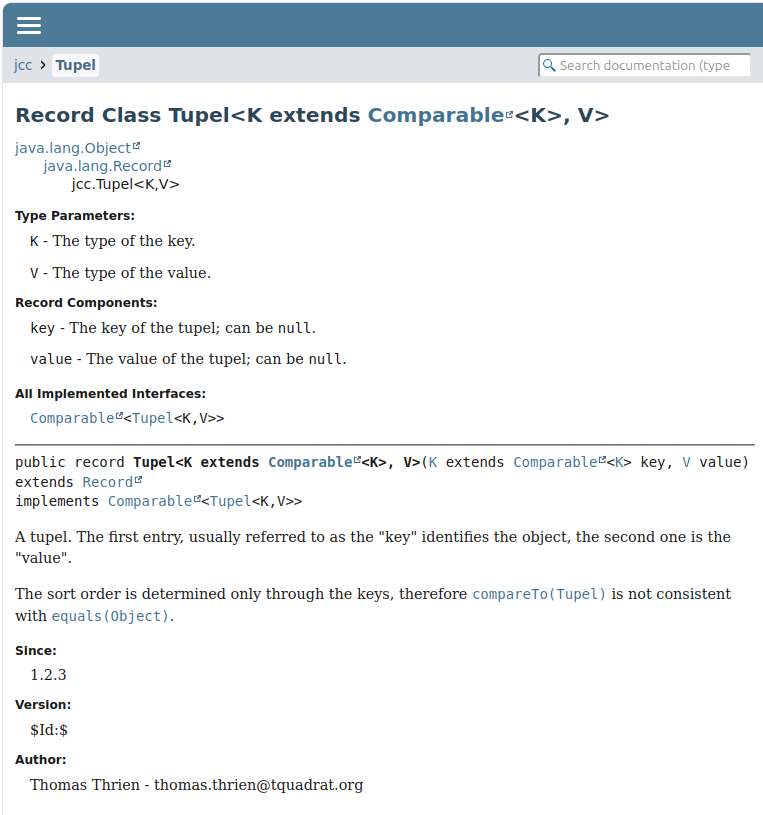
\includegraphics[scale=0.55]{comments/JavadocTupel1}
\end{center}

\clearpage
Despite none of the methods\index{method} nor the constructor\index{constructor} were explicitly defined, they are listed for the \lstinline|Tupel| record class\index{record}, even with a meaningful description:
\begin{center}
	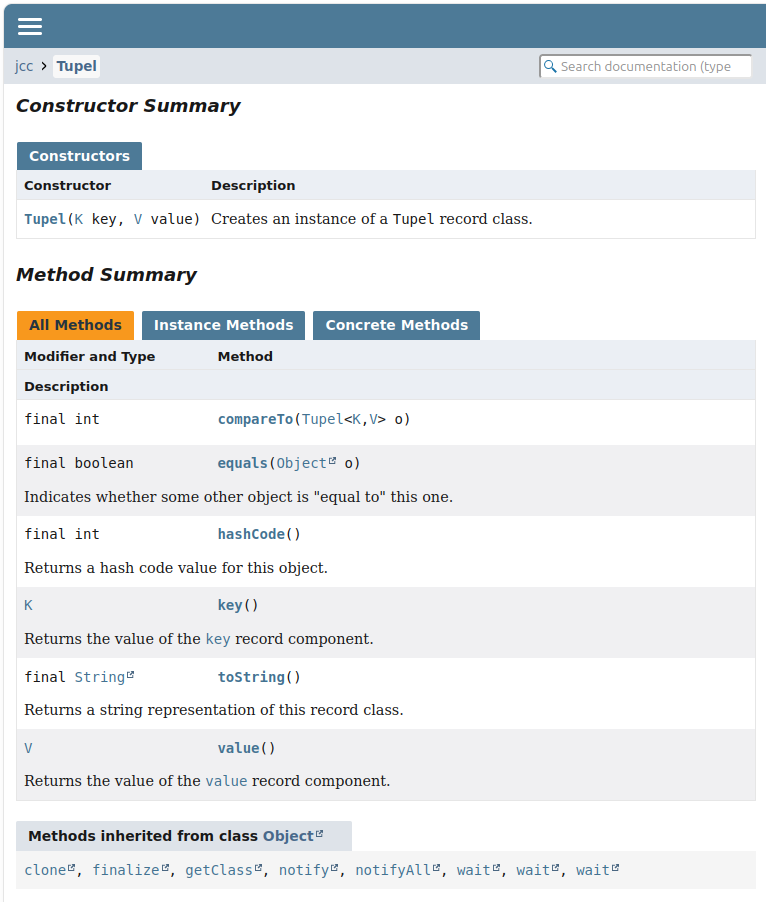
\includegraphics[scale=0.55]{comments/JavadocTupel2}
\end{center}
That there is no description for \lstinline|compareTo()| is due to a bug in the Javadoc tool in the version used for the generation; usually, the documentation is inherited from the overridden method\index{method!overridden method}. At the very least, the Javadoc tool\index{javadoc} generated the link to the documentation of the overridden method\index{method!overridden method} within the method's detailed documentation:
\begin{center}
	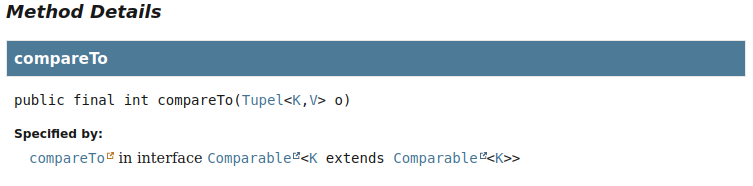
\includegraphics[scale=0.55]{comments/JavadocTupel3}
\end{center}

%==============================================================================
% End of file!!
%==============================================================================

\subsection{The Field Comment}\label{sec:FieldComment}
Attributes/properties\index{field!attribute}\index{property}, constants\index{field!constant} and \lstinline|enum|\index{enum} values are all summarised under \bsq{field}\index{field} here.

Each and every field\index{field} must have a comment, the \bsq{field comment}, describing it. For private fields\index{field} it can be sufficient to refer to the related getter method\index{method!getter method}\footnote{Of course you have to provide a complete documentation of the property\index{property} there; just a line with a \bdq{\{\nameref{sec:TagReturn} …\}}\index{return@"@return} inline tag will not do the job for the getter method\index{method!getter method} in this case.} instead of writing a lengthy comment into the field comment itself; but do not use the \bdq{\nameref{sec:TagSee}}\index{see@"@see} tag instead of the \bdq{\{\nameref{sec:TagLink} …\}}\index{link@"@link} tag:
\begin{lstlisting}
/**
 *  <p>{@summary For the description of the property 'value' refer to
 *  {@link #getValue()}.
 */
private final Value m_Value;

// AVOID!! Do not use @see
/**
 *  @see #getOtherValue()}.
 */
private final Value m_OtherValue;
\end{lstlisting}

If there is no getter method\index{method!getter method} for the field\index{field}, or if it is not private, a proper description is mandatory. One sentence is enough in most cases, but you are not limited to that.

It is always a good idea to describe the valid values for the field\index{field}, its default value, and whether \lstinline|null| is a possible value for a reference. This is a hard requirement for all non-final non-private fields\index{field} – in particular because there should \textit{never} be any non-final non-private fields\index{field} at all!

For a serialisable class\index{class}\index{serialization}, the fields\index{field} that will be serialised should be tagged with \bdq{\nameref{sec:TagSerial}}\index{serial@"@serial} and the appropriate description.

% Elaborate on comments for constants!!!!





Constants (\lstinline|public static final| fields) that are initialised with a literal have to use the \nameref{sec:TagValue} tag in there description. Also \lstinline|private static final| or \lstinline|protected static final| fields that are initialised with a literal should use the \nameref{sec:TagValue}.

This looks like this:
\begin{lstlisting}
/**
 *  The vested system property for the file encoding used by the JVM:
 *  {@value}.
 */
public static final String PROPERTY_FILE_ENCODING = "file.encoding";
\end{lstlisting}

The comments for enum values are nothing else than field comments for constants – in fact, an enum value is exactly that: a \lstinline|public static final| field initialised with an instance of the enum type.


%==============================================================================
% End of file!!
%==============================================================================



%==============================================================================
% End of file!!
%==============================================================================

\section{Additional Files}\label{sec:AdditionalFiles}
In any documentation comment you can add references to external locations for additional information through the HTML\index{HTML} \lstinline|<href>| tag:
\keeplisting{3}
\begin{lstlisting}[language=Comment]
…
*  For additional information, refer to 
*  <href a="https://stackoverflow.com/">Stack Overflow</href>.
…  
\end{lstlisting}

Or you use the custom tag \bdq{\{\nameref{sec:TagHref}\}} for that purpose:
\keeplisting{3}
\begin{lstlisting}[language=Comment]
…
*  For additional information, refer to 
*  {@href https://stackoverflow.com/ Stack Overflow}.
…  
\end{lstlisting}
The output will be the same in both cases.

Additional data (screenshots, images, charts, texts, sample code, scripts,~…) that is not available through an URL or should not be accessed from the network can be added to the generated documentation. The respective files will be placed to a \bdq{\texttt{doc-files}}\index{doc-files} subfolder that can be added to each package\index{package} folder. HTML\index{HTML} and Markdown\index{Markdown} files are parsed by the Javadoc\index{javadoc} tool, meaning that you can use the Javadoc\index{javadoc} tag in there.

% How to refer to the doc-files?
% Images??

%==============================================================================
% End of file!!
%==============================================================================


\section{The Javadoc Tags}\label{sec:JavaDocTags}
The Javadoc\index{javadoc} tool comes with a set of tags that help to create compile documentation comments that generate neatly to a useful documentation of the product.

\Java also provides an API for custom tags  \autocite{ORACLE_DOC_TAGLET_INTERFACE}; it even provides an API  \autocite{ORACLE_DOC_DOCLET_PACKAGE,ORACLE_DOC_DOCLET_INTERFACE} that allows to customize the complete generation process.

%------------------------------------------------------------------------------

\subsection{The Standard Doclet Tags}
Most of the contents of this chapter is quoted from the document \bdq{JavaDoc Documentation Comment Specification for the Standard Doclet (JDK 25)} \autocite{ORACLE_DOC_JAVADOC_TAG}. 

The output of the Javadoc\index{javadoc} tool is determined by the implementation of the interface \lstinline|jdk.javadoc.doclet.Doclet| \autocite{ORACLE_DOC_DOCLET_INTERFACE} that is specified on the command line for \texttt{javadoc} by the options \texttt{-doclet} and \texttt{-docletpath} \autocite{ORACLE_TOOL:javadoc:options}. The \lstinline|Doclet| implementation is also responsible for interpreting the content of the documentation comments.

If no explicit \lstinline|Doclet| class is specified on the command line, the standard doclet (provided through the class \lstinline|jdk.javadoc.doclet.StandardDoclet| \autocite{ORACLE_DOC_STANDARDDOCLET_CLASS}) is used; it understands the Javadoc tags described below, and it provides an API for additional tags.

Alternative implementations for the \lstinline|Doclet| interface may accept the same syntax as the standard doclet, they may handle the tags completely different or they can ignore them completely. However, due to the support by many tools, the syntax supported by the standard doclet has become a \textit{de facto} standard.

%--------------------------------------------------------------------

\paragraph{\lstinline|@author|}\label{sec:TagAuthor}\index{author@"@author} Usage: \lstinline|@author <name-text>|

The tag adds an \bdq{\textsf{Author:}} entry with the specified name to the generated documentation when the \texttt{-author} option is specified on the command line for the Javadoc\index{javadoc}. A documentation comment can contain multiple \nameref{sec:TagAuthor} tags. Consider to use the custom \bdq{\nameref{sec:TagExtAuthor}}\index{extauthor@"@extauthor}  tag instead.

%--------------------------------------------------------------------

\paragraph{\lstinline|@code|}\label{sec:TagCode}\index{code@"@code}  Usage: \lstinline|{@code <text>}|

This is equivalent to \lstinline|<code>{@literal text}</code>|.

It displays text in the code font without interpreting the text as HTML\index{HTML} markup or nested Javadoc tags. This enables you to use regular angle brackets (\bdq{\textless} and \bdq{\textgreater}) instead of the HTML\index{HTML} entities (\texttt{\&lt;} and \texttt{\&gt;}) in documentation comments, such as in parameter types (\texttt{<Object>}), inequalities ($3 < 4$), or arrows (\texttt{-\textgreater}).

Use the \bdq{\{\nameref{sec:TagLiteral} …\}}\index{literal@"@literal} tag if you want the same functionality without the code font. 

%--------------------------------------------------------------------

\paragraph{\lstinline|@deprecated|}\index{deprecated@"@deprecated}  Usage: \lstinline|@deprecated <text>|

This tag is used in conjunction with the \lstinline|@Deprecated| \autocite{ORACLE_DOC_DEPRECATED_ANNOTATION} annotation to indicate that this API should no longer be used (even though it may continue to work).

The first sentence of the text should tell the user when the API was deprecated and what to use as a replacement. Subsequent sentences can also explain why it was deprecated.

A \bdq{\{\nameref{sec:TagLink} …\}}\index{link@"@link} tag that points to the replacement API should be added where feasible.


%--------------------------------------------------------------------

\paragraph{\lstinline|@docRoot|}  Usage: \lstinline|{@docRoot}|

Represents the relative path to the generated document's (destination) root directory from any generated page. This tag is useful when you want to include a file, such as a copyright page or company logo, that you want to reference from all generated pages.

%--------------------------------------------------------------------

\paragraph{\lstinline|@exception|} This is a synonym for the \bdq{\nameref{sec:TagThrows}}\index{throws@"@throws} tag; it should not be used.

%--------------------------------------------------------------------

\paragraph{\lstinline|@hidden|}\index{hidden@"@hidden}  Usage: \lstinline|@hidden|

Hides a program element from the generated API documentation. This tag may be used when it is not otherwise possible to design the API in a way that such items do not appear at all.

%--------------------------------------------------------------------

\paragraph{\lstinline|@index|}\index{index@"@index}  Usage: \lstinline|{@index <word> <description>}| or\\  
\lstinline|    {@index "<phrase>"  <description>}|

Declares that a word or phrase, together with an optional short description, should appear in the index files generated by the standard doclet. The index entry will be linked to the word or phrase that will appear at this point in the generated documentation. The description may be used when the word or phrase to be indexed is not clear by itself, such as for an acronym.

%--------------------------------------------------------------------

\paragraph{\lstinline|@inheritDoc|}\label{sec:TagInheritDoc}  Usage: \lstinline|{@inheritDoc}|

Inherits (copies) the documentation comment from the nearest inheritable class or implementable interface into the current documentation comment at this tag's location. This enables you to write more general comments higher up the inheritance tree and to write around the copied text.

\paragraph{\lstinline|@link|}\label{sec:TagLink}  Usage: \lstinline|{@link <module/package.class#member> <label>}|

Inserts an inline link with a visible text label that points to the documentation for the specified module, package, class, or member name of a referenced class. 

This tag is similar to the \nameref{sec:TagSee} tag. Both tags require the same references and accept the same syntax for \verb|<module/package.class#member>| and the label. The main difference is that the \lstinline|{@link}| tag generates an inline link rather than placing the link in the “See Also” section. The \lstinline|{@link}| tag begins and ends with curly braces to separate it from the rest of the inline text. If you need to use the right curly brace (“\}”) inside the label, then use the HTML entity notation \verb|&#125;|.

\paragraph{\lstinline|@linkplain|}\label{sec:TagLinkplain}  Usage: \lstinline|{@linkplain <module/package.class#member> <label>}|

Behaves the same as the \nameref{sec:TagLink} tag, except the link label is displayed in plain text rather than code font. Useful when the label is plain text.

\paragraph{\lstinline|@literal|}\label{sec:TagLiteral}  Usage: \lstinline|{@literal <text>}| 

Same as the \nameref{sec:TagCode} tag, but the text is shown as plain text and not in the code font.

\paragraph{\lstinline|@param|}\label{sec:TagParam}  Usage: \lstinline|@param <parameter-name> <description>|

Adds a parameter with the specified parameter name followed by the specified description to the “Parameters” section. The parameter name can be the name of a parameter in a method or constructor, or the name of a type parameter of a class, method, or constructor. Use angle brackets (“\verb#<…>#”) around such a parameter name to indicate the use of a type parameter.

\paragraph{\lstinline|@provides|}\label{sec:TagProvides}  Usage: \lstinline|@provides <service-type> <description>|

This tag may only appear in the documentation comment inside a \verb#module-info.java# file. It serves to document an implementation of a service that is provided by the module. The description may be used to specify how to obtain an instance of this service provider, and any important characteristics of the provider itself. 

\paragraph{\lstinline|@return|}\label{sec:TagReturn}  Usage: \lstinline|@return <description>|

Adds a “Returns” section with the description text to the documentation comment of a method.

\paragraph{\lstinline|@see|}\label{sec:TagSee}  Adds a “See Also” heading with a link or text entry that points to a reference. The \lstinline|@see| tag has three variations; see \autocite{ORACLE_DOC_JAVADOC_TAG} for the details.

\paragraph{\lstinline|@serial|}\label{sec:TagSerial} Used in the documentation comment for a default serializable field. See “Documenting Serializable Fields and Data for a Class”\autocite{ORACLE_DOC_OBJECT_SERIALIZATION:DocumentingSerializableFieldsData}. 

\paragraph{\lstinline|@since|}\label{sec:TagSince}  Usage: \lstinline|@since <since-text>|

Adds a “Since” heading with the specified \verb#<since-text># value to the generated documentation. The text has no special internal structure. This tag that this change or feature has existed since the software release specified by the \verb#<since-text># value, for example: \lstinline|@since 1.5|.

Although it would possible to provide a date or something else, it is recommended to always use a version number with the \lstinline|@since| tag.

\paragraph{\lstinline|@summary|}\label{sec:TagSummary}  Usage:  \lstinline|{@summary <text>}|

Identifies  the summary of an API description, as an alternative to the default policy to identify and use the first sentence of the API description. The tag only has significance when used at the beginning of a description. In all cases, the tag is rendered by simply rendering its content.

The \lstinline|{@summary}| tag has to be used always when a documentation comment has more than one sentence; see also chapter \tqvref{sec:StructureAndContents}.

\paragraph{\lstinline|@throws|}\label{sec:TagThrows}  Usage: \lstinline|@throws <class-name> <description>|

The \lstinline|@throws| tag adds a “Throws” subheading to the generated documentation, with the \verb#<class-name># and the description text. The class name is the name of the exception that might be thrown by the method, and the description provides information about the conditions for that exception to be thrown. 

\paragraph{\lstinline|@uses|}\label{sec:TagUses}  Usage: \lstinline|@uses <service-type> <description>|

This tag may only appear in the documentation comment inside a \verb#module-info.java# file. It serves to document that a service may be used by the module. The description may be used to specify the characteristics of the service that may be required, and what the module will do if no provider for the service is available.

\paragraph{\lstinline|@value|}\label{sec:TagValue}  Usage: \lstinline|{@value}| or \lstinline|{@value <module/package.class#field>}|

This tag is used to display the values of constant in the generated documentation. When the \lstinline|{@value}| tag is used without an argument in the documentation comment of a \lstinline|static final| field, it displays the value of that constant:
\begin{lstlisting}
/**
 * The value of this constant is {@value}.
 */
public static final String SCRIPT_START = "<script>"
\end{lstlisting}

When used with the argument \verb|<module.package.class#field>| in any documentation comment, the \lstinline|{@value}>| tag displays the value of the specified constant:
\begin{lstlisting}
/**
 * Evaluates the script starting with {@value #SCRIPT_START}.
 */
public final String evalScript( String script ) { … }
\end{lstlisting}
The argument \verb|<module.package.class#field>| takes a form similar to that of the \nameref{sec:TagLink}, the \nameref{sec:TagLinkplain}, or the \nameref{sec:TagSee} tag argument, except that the member always must be a \lstinline|static final| field.

\paragraph{\lstinline|@version|}\label{sec:TagVersion}  Usage: \lstinline|@version <version-text>|

Adds a “Version” subheading with the specified \verb#<version-text># value to the generated documents when the \verb#-version# option is specified on the command line. This tag is intended to hold the current release number of the software that this code is part of, as opposed to the \nameref{sec:TagSince} tag, which holds the release number where this code was introduced. The \verb#<version-text># value has no special internal structure.

%==============================================================================
% End of file!!
%==============================================================================


\subsection{Custom Tags for JavaDoc}\label{sec:CustomTagsForJavaDoc}
The Javadoc\index{javadoc} tool allows to add custom tags that can be used within the documentation comments.

There are two different ways to add custom tags. The easier one is to configure them just on the command line for the tool, the more flexible one requires to write Java code that implements the \lstinline|jdk.javadoc.doclet.Taglet|\index{jdk.javadoc.doclet!Taglet} \autocite{ORACLE_DOC_TAGLET_INTERFACE} interface.

\subsubsection{Simple Custom Tags}\label{sec:SimpleCustomTags}
A simple custom tag is configured completely on the command line for the invocation of the Javadoc\index{javadoc} tool. This approach allows only block tag, but the text for these tags comes with full support for all inline tags.

\keeplisting{2}
The command line option for a new simple custom tag looks like this:
\begin{lstlisting}[numbers=none,language={}]
-tag <name>[:[<locations>]:<header>]
\end{lstlisting}

This specifies a custom block tag \texttt{<name>}. For the Javadoc\index{javadoc} tool to spell-check tag names, it is important to include a \texttt{-tag} option for every custom tag that is present in the source code, disabling (with \texttt{X} as the location) those that aren't being output in the current run.

\texttt{<locations>} is a combination of the letters below, in either uppercase or lowercase, that determine where the custom tag is allowed:
\begin{itemize}[nosep]
	\item{\texttt{A}: all declarations}
	\item{\texttt{C}: constructors\index{constructor}}
	\item{\texttt{F}: fields\index{field}}
	\item{\texttt{M}: methods\index{method}}
	\item{\texttt{O}: the overview page and other documentation files in doc-files subdirectories}
	\item{\texttt{P}: packages\index{package}}
	\item{\texttt{S}: modules\index{module}}
	\item{\texttt{T}: types (classes\index{class} and interfaces\index{interface})}
	\item{\texttt{X}: nowhere: the tag is disabled, and will be ignored, together with its argument}
\end{itemize}

Finally, \texttt{<header>} is the tag heading that is rendered in bold, followed by the tag's single argument in the next line.

\keeplisting{2}
For the command line option
\begin{lstlisting}[numbers=none,language={}]
-tag implNote:a:Implementation Note:
\end{lstlisting}
and the source code below
\keeplisting{10}
\begin{lstlisting}
/**
 *  {@summary Retrieves data from the queue.}
 *  
 *  @param  <T> The type of the data in the queue.
 *  @param  queue   The queue.
 *  @return An instance of
 *      {@link Optional}
 *      that holds the retrieved data.
 *  
 *  @implNote The method may not block; if the queue is (currently) empty,
 *      the implementation must return
 *      {@linkplain Optional#empty() empty}.
 */
public <T> T retrieveData( final Queue<T> queue );
\end{lstlisting}
the output will look like this:
\begin{center}
	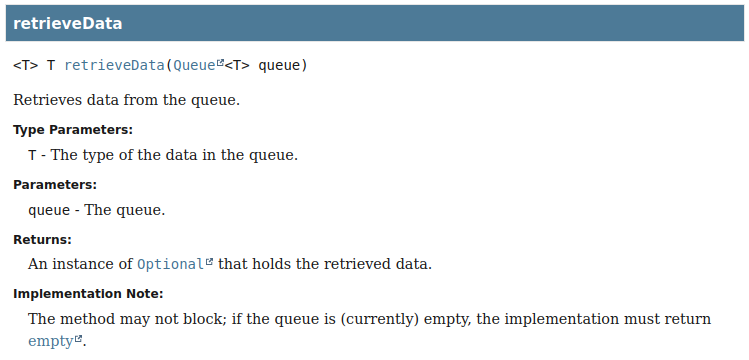
\includegraphics[scale=0.55]{comments/JavadocCustomTag1}
\end{center}

The colon (\bdq{:}) is always the separator. To include a colon in the tag name, escape it with a backslash. Omitting a value for \texttt{<header>} causes the name to be the heading, and if no location is specified, the tag can be used everywhere (same as \texttt{A} was specified). Refer also to \autocite{ORACLE_DOC_JAVADOC_MAN:StandardDocletOptions}.

The three tags below are defined per convention and widely used throughout the official documentation of the \Java API:

\paragraph{\lstinline|@apiNote|}\label{sec:TagApiNote}\index{apiNote@"@apiNote} Usage: \lstinline|@apiNote <text>|

This tag is used to provided some notes regarding the API.

\paragraph{\lstinline|@implNote|}\label{sec:TagImplNote}\index{implNote@"@implNote} Usage: \lstinline|@implNote <text>|

With this tag, you can add notes on how an implementation looks like (or should look like) to a program element.

\paragraph{\lstinline|@implSpec|}\label{sec:TagImplSpec}\index{implSpec@"@implSpec} Usage: \lstinline|@implSpec <text>|

This tag is added to provide information about the specification that is the base of the implementation for the respective program element.

\keeplisting{4}
To use these tags, they must be registered on the command line like this:
\begin{lstlisting}[numbers=none,language=sh]
javadoc -tag apiNote:a:API Note: \
        -tag implSpec:a:Implementation Requirements: \
        -tag implNote:a:Implementation Note:
\end{lstlisting}

%------------------------------------------------------------------------------

\subsubsection{Custom Taglets}\label{sec:CustomTaglets}
An introduction to implementing custom taglets would go beyond the scope of this book. However, the documentation for the \lstinline|jdk.javadoc.doclet.Taglet|\index{jdk.javadoc.doclet!Taglet} \autocite{ORACLE_DOC_TAGLET_INTERFACE} already provides a useful starting point.

Custom taglets do allow also the implementation of inline tags, on the other hand, they do not support to include the already existing inline tags.

If you want to use custom taglets, you have to provide the path to the implementing classes with the command line option \mbox{\texttt{-tagletpath}}; multiple locations are separated by a colon (\bdq{:}) on Linux/Unix operating systems, or by a semi-colon (\bdq{;}) on Windows.

Next each Taglet implementation class needs to be registered with the command line option \mbox{\texttt{-tagletclass}} (one entry per class).

I created a set of custom tags that I use regularly, and that I also recommend for your documentation comments. The respective library (\bdq{tquadrat’s Javadoc Extensions} or short \bsq{foundation-javadoc}) can be found at \autocite{TQUADRAT_ORG_FOUNDATION_JAVADOC}.

The command line for this would look like this:\footnote{Check the project's website at \autocite{TQUADRAT_ORG_FOUNDATION_JAVADOC} for the current version.}
\keeplisting{20}
\begin{lstlisting}
-tagletpath /path/to/org.tquadrat.foundation.javadoc-0.25.4.jar:\
/path/to/apiguardian-api-1.1.2.jar:/path/to/jakarta.activation-2.0.1.jar \
\
-taglet org.tquadrat.foundation.javadoc.AnchorTaglet \
-taglet org.tquadrat.foundation.javadoc.AuthorTaglet \
-taglet org.tquadrat.foundation.javadoc.FALSETaglet \
-taglet org.tquadrat.foundation.javadoc.HRefTaglet \
-taglet org.tquadrat.foundation.javadoc.IgnoreTaglet \
-taglet org.tquadrat.foundation.javadoc.ImageTaglet \
-taglet org.tquadrat.foundation.javadoc.IncludeTaglet \
-taglet org.tquadrat.foundation.javadoc.InspiredTaglet \
-taglet org.tquadrat.foundation.javadoc.ModifiedTaglet \
-taglet org.tquadrat.foundation.javadoc.NoteTaglet \
-taglet org.tquadrat.foundation.javadoc.NULLTaglet \
-taglet org.tquadrat.foundation.javadoc.ThanksTaglet \
-taglet org.tquadrat.foundation.javadoc.ToDoTaglet \
-taglet org.tquadrat.foundation.javadoc.TRUETaglet \
-taglet org.tquadrat.foundation.javadoc.UmlGraphLinkTaglet \
-taglet org.tquadrat.foundation.javadoc.UnderlineTaglet \
\
-tag hidden -tag note -tag param -tag return -tag throws -tag author -tag extauthor -tag thanks -tag modified -tag version -tag since -tag see -tag inspired -tag spec -tag provides -tag uses -tag UMLGraph.link -tag deprecated -tag todo \
-tag apiNote:a:API Note: \ 
-tag implSpec:a:Implementation Requirements: \
-tag implNote:a:Implementation Note: 
\end{lstlisting}

The purpose of the \texttt{-tag} options here is to determine the order in which the block tags appear in the final documentation. The command line for the Javadoc\index{javadoc} tool is further discussed in chapter \tqfullref{sec:RunJavadoc}.

\bdq{tquadrat’s Javadoc Extensions} provides the following custom taglets:

\keeplisting{4}
\paragraph{\lstinline|@anchor|}\label{sec:TagAnchor}  Usage: \lstinline|{@anchor #<anchor-name> <text>}|

This tag allows to add an HTML anchor to the generated documentation, where \texttt{\#<anchor-name>} is the name of the anchor to the given text. The hash symbol (\bsq{\#}) before the name of the anchor is mandatory!

%------------------------------------------------------------------------------

\keeplisting{5}
\paragraph{\lstinline|@author|}\label{sec:TagExtAuthor}  Usage: \lstinline|@author <name-text> - <email-address>| or \\
\lstinline|    @extauthor <name-text> - <email-address>|

This is a replacement for the \nameref{sec:TagAuthor}\index{author@"@author} tag that renders the given email address as a \texttt{mailto:} link in the generated documentation. It does not regard the option \mbox{\texttt{-author}} on the command line\footnote{This is valid for the current version 0.25.4 of the library; it may have changed for a later version.}.

The \lstinline|@extauthor| was introduced because some versions of the Javadoc\index{javadoc} did not allow to overwrite the standard \nameref{sec:TagAuthor}\index{author@"@author} tag.

%------------------------------------------------------------------------------

\paragraph{\lstinline|@false|}\label{sec:TagFALSE}  Usage: \lstinline|{@false}|

This is a shortcut for \lstinline|{@code false}|\index{code@"@code}.

%------------------------------------------------------------------------------

\paragraph{\lstinline|@href|}\label{sec:TagHref}  Usage: \lstinline|{@href <url> <text>}| or \lstinline|{@href <url>}|

With this tag, an HTML hyperlink can be added to the generated documentation; it will be placed inside the description text, but different from the \nameref{sec:TagLink} and \nameref{sec:TagLinkplain} tags, it allows to refer to arbitrary external resources, not only to other documented elements. Obviously, \texttt{<url>} is the target URL, while \texttt{<text>} is the clickable text. If the latter is omitted, the URL itself will be used instead.

%------------------------------------------------------------------------------

\paragraph{\lstinline|@ignore|}\label{sec:TagIgnore}  Usage: \lstinline|{@ignore <text>}|

With this tag text can be added to the documentation comment that is not shown in the generated documentation.

%------------------------------------------------------------------------------

\paragraph{\lstinline|@image|}\label{sec:TagImage}  Usage: \lstinline|{@image <url> <attributes>}|

The tag allows to add a picture to the generated documentation. \texttt{<url>} is the location of the image file, while \texttt{<attributes>} are HTML\index{HTML} attributes that are allowed for the \lstinline|<img>| tag.

%------------------------------------------------------------------------------

\paragraph{\lstinline|@include|}\label{sec:TagInclude}  Usage: \lstinline|{@include <source>:<process-mode>|

This tag allows you to include the contents of an external file in different ways, determined by the \texttt{<process-mode>}. It can be used to embed source code snippets into the documentation, but also to load text modules. 

\keeplisting{5}
Valid values for \texttt{<process-mode>} are:
\begin{itemize}[nosep]
	\item PLAIN
	\item ESCAPE
	\item MARKDOWN
	\item SOURCE
\end{itemize}

The code below includes the contents of the same file:
\keeplisting{8}
\begin{lstlisting}[language=Comment]
 …
 *  <hr>
 *  <p>{@include ${includes}/sample.html:PLAIN}</p>
 *  <hr>
 *  <p>{@include ${includes}/sample.html:ESCAPE}</p>
 *  <hr>
 *  <p>{@include ${includes}/sample.html:SOURCE}</p>
 *  <hr>
 …
\end{lstlisting}

For \bdq{\texttt{<process-mode> = PLAIN}} the output looks like this: 
\begin{center}
	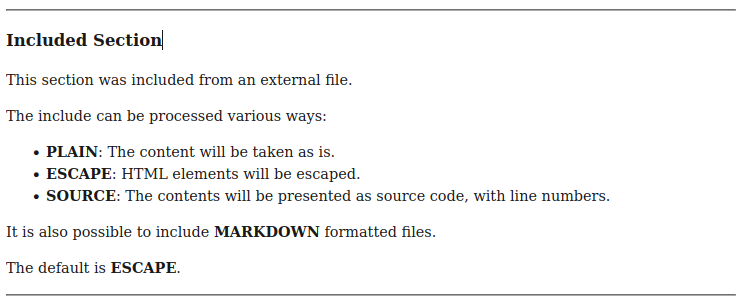
\includegraphics[scale=0.55]{comments/JavadocIncludePlain}
\end{center}
\bdq{\texttt{<process-mode> = ESCAPE}} is rendered like this: 
\begin{center}
	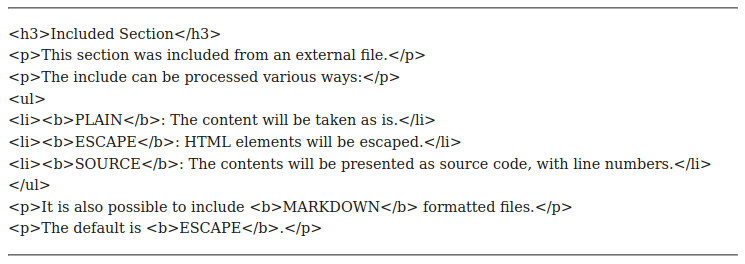
\includegraphics[scale=0.55]{comments/JavadocIncludeEscape}
\end{center}
And \bdq{\texttt{<process-mode> = SOURCE}} results a below: 
\begin{center}
	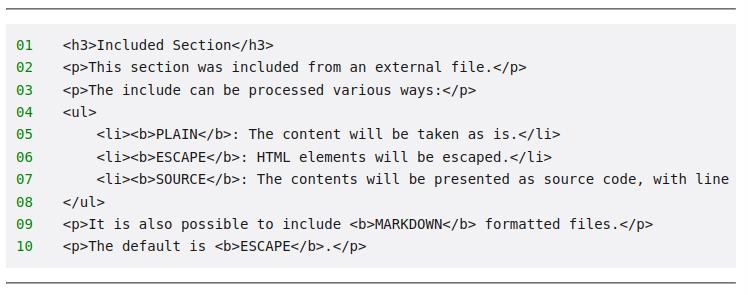
\includegraphics[scale=0.55]{comments/JavadocIncludeSource}
\end{center}

For more details on the \bdq{\{\nameref{sec:TagInclude}\}} tag, refer to \autocite{TQUADRAT_ORG_FOUNDATION_JAVADOC}.

%------------------------------------------------------------------------------

\paragraph{\lstinline|@inspired|}\label{sec:TagInspired}  Usage: \lstinline|@inspired <text>|

Sometimes a piece of code was inspired by a document of some kind, a description of an algorithm, a product white paper, or whatever. This tag allows you to add a reference to that source of inspiration.

Refer also to \nameref{sec:TagSpec}\index{spec@"@spec}, \nameref{sec:TagImplNote}\index{implNote@"@implNote}, \nameref{sec:TagImplSpec}\index{implSpec@"@implSpec} and \nameref{sec:TagApiNote}\index{apiNote@"@apiNote} as they are somehow related. In particular if the reference to the inspiration is only a URL, the \nameref{sec:TagSpec}\index{spec@"@spec} is preferred.

%------------------------------------------------------------------------------

\paragraph{\lstinline|@modified|}\label{sec:TagModified}  Usage: \lstinline|@modified <name-text> - <email-address>|

This is a variant of the \nameref{sec:TagExtAuthor} tag. It is meant to provide the name of the developer that modified the respective element without claiming to be an author.

%------------------------------------------------------------------------------

\paragraph{\lstinline|@note|}\label{sec:TagNote}  Usage: \lstinline|@note <text>|

With this tag, it is easy to add important notes to the generated documentation for an element. All notes will be added to a bullet list placed immediately beneath the documentation text. The text for the \lstinline|@note| tag is somehow limited as it does not allow other Javadoc tags.

%------------------------------------------------------------------------------

\paragraph{\lstinline|@null|}\label{sec:TagNULL}  Usage: \lstinline|{@null}|

This is a shortcut for \lstinline|{@code null}|\index{code@"@code}.

%------------------------------------------------------------------------------

\paragraph{\lstinline|@thanks|}\label{sec:TagThanks}  Usage: \lstinline|@thanks <name-text> - <email-address>|

Use this tag to mention someone who provided input to the respective element without being an author; that person might have wrote an article about the algorithm that was implemented by this element, or they may have reported a bug.

Same as for the \nameref{sec:TagExtAuthor} and the \nameref{sec:TagModified} tags, the email address will be rendered to a \verb#mailto:# link in the generated documentation.

%------------------------------------------------------------------------------

\paragraph{\lstinline|@todo|}\label{sec:TagTodo}  Usage: \lstinline|@todo <todo.md>|

This tag copies the contents of the Markdown\index{Markdown} file specified by \texttt{<todo.md>} into the generated documentation. This is meant as a ToDo list or list of open issues, and that is reflected by the heading that is added to the generated documentation.

%------------------------------------------------------------------------------

\paragraph{\lstinline|@true|}\label{sec:TagTRUE}  Usage: \lstinline|{@true}|

This is a shortcut for \lstinline|{@code true}|\index{code@"@code}.

%------------------------------------------------------------------------------

\paragraph{\lstinline|@UMLGraph.link|}\label{sec:TagUMLGraph}  Usage: \lstinline|@UMLGraph.link|

This adds an UML graph for the current class to the generated documentation.

%------------------------------------------------------------------------------

\paragraph{\lstinline|@underline|}\label{sec:TagUnderline}  Usage: \lstinline|{@underline <text>}|

Use this tag to add underlined text to the generated documentation.

%==============================================================================
% End of file!!
%==============================================================================



%==============================================================================
% End of file!!
%==============================================================================


\section{Tips and Tricks}
\subsection{Special Characters}\label{sec:DocCommentSpecialChars}
The documentation comments are parsed by the Javadoc\index{javadoc} tool and then translated to HTML\index{HTML}. During that process, the comments will be scanned for the various Javadoc tags, mentioned \hyperref[sec:JavaDocTags]{above}. Additionally, the DocLint feature validates the output as proper HTML5\index{HTML}.

If you need to use the right curly brace (\bdq{\}}) inside the link label, then use the HTML entity notation \texttt{\&\#125;}.

\bdq{\{\nameref{sec:TagLiteral} …\}}\index{literal@"@literal}
\bdq{\{\nameref{sec:TagCode} …\}}\index{code@"@code}

\lipsum(1)
\subsection{Embedding Code Snippets}\label{sec:EmbeddingCodeSnippets}

\bdq{\{\nameref{sec:TagSnippet} …\}}\index{snippet@"@snippet}

\autocite{JEP413}
\autocite{Baeldung:CodeSnippets}  \autocite{ORACLE_DOC_JAVADOC_GUIDE:Snippets}  \autocite{Korando:CodeSnippets} 

\lipsum(1)
\subsection{IDE Support}
Eclipse can be configured in a way that it will issue warnings or even errors for missing documentation comments: see \texttt{Window | Preferences | Java | Compiler | Javadoc}.

To achieve the same for IntelliJ IDEA, you go to \texttt{File | Settings}, and there you select \texttt{Editor | Inspections > Java > Javadoc}.

%==============================================================================
% End of file!!
%==============================================================================

\section{Generate the Documentation}\label{sec:RunJavadoc}
In this chapter, we will discuss the command line options for the Javadoc\index{javadoc}, based on the documentation that can be found at \autocite{ORACLE_DOC_JAVADOC_MAN}. That assumes that you start \lstinline|javadoc|\index{javadoc} from the command line directly.

Alternatively, you can launch it through Ant\index{Apache Ant}\index{ant|see {Apache Ant}} \autocite{APACHE_ANT}, Gradle\index{Gradle} \autocite{GRADLE} or Maven\index{Apache Maven} \autocite{APACHE_MAVEN}, or you can even write your own starter program. But the command line options will remain the same, although they may be hidden behind some other names; the documentation of the respective tool will help here:

\begin{itemize}
	\item{for Ant\index{Apache Ant} see \autocite{APACHE_ANT:Javadoc}}
	\item{for Gradle\index{Gradle} see \autocite{GRADLE:Javadoc}}
	\item{for Maven\index{Apache Maven} see \autocite{APACHE_MAVEN:Javadoc}}
\end{itemize}

If you start \lstinline|javadoc|\index{javadoc} from the command line, I recommend to write all command line options to an \bsq{\texttt{options}} file that you refer to with the \verb#@# option:
\begin{lstlisting}[numbers=none,language=sh]
javadoc @options @packages @sources -d <destination-folder>
\end{lstlisting}

For this command line, the \bsq{\texttt{packages}} file would contain the packages that should be considered for the documentation, and the \bsq{\texttt{sources}} file contains the source directories. \bsq{\texttt{<destination-folder>}} is the target for the generated documentation.

\subsubsection{Scope of the generated Documentation}\label{sec:GenerationScope}
The scope of the generated documentation depends on the type of product you have to deliver (refer to \tqfullvref{sec:TypesOfProducts}) and the audience for that documentation.

The table below shows the command line options that determine the volume of the generated documentation for the product types and audiences.

\renewcommand{\cellalign}{tl}
\LTXtable{\linewidth}{comments/Scope.tbl.tex}

For a function library\index{product type!function library}, the \bdq{users} are external developers that integrate that library into their product. That is slightly different for a feature library\index{product type!feature library}: the users will just add the library, while external developers dig deeper (admittedly, this distinction is rather arbitrary).

For tools\index{product type!tool}, extensions\index{product type!extension}, standalone\index{product type!standalone application} and server-based applications\index{product type!server-based application}, no Javadoc\index{javadoc} documentation will be generated for the public. Only when a standalone application\index{product type!standalone application} allows customisation, it may make sense to generate a Javadoc\index{javadoc} documentation for the public API that can be used by external developers for the customisations.

For server-based applications\index{product type!server-based application} and extension\index{product type!extension}, a generated documentation is usually also not useful.

The meaning of the command line options is described below:

\paragraph{\texttt{-author}} If set, the value of the \nameref{sec:TagAuthor} tag will be included into the generated documentation. It might be omitted for documentation meant for the public.

\paragraph{\texttt{-{}-expand-requires}} Instructs the Javadoc\index{javadoc} tool to expand the set of modules to be documented. If not set, only the modules given explicitly on the command lin are documents. With the argument \bsq{\texttt{transitive}}, all the required transitive dependencies of those modules are included, and the argument \bsq{\texttt{all}} includes all dependencies. 

\paragraph{-nodeprecated} Prevents the generation of the documentation for any deprecated element. It might by useful for function\index{product type!function library} and feature libraries\index{product type!feature library} when you want to prevent that deprecated APIs are still used. 

\paragraph{-notimestamp} Supresses the time stamp, which is hidden in an HTML\index{HTML} comment in the generated documentation.

\paragraph{\texttt{-private}, \texttt{-protected}, \texttt{-public}} These three options\footnote{There is also a fourth one, \mbox{\bsq{\texttt{-package}}}, that is usually not used.} controls what is shown in the generated documentation: if \mbox{\bsq{\texttt{-private}}} is set, all classes and members are part of the documentation, \mbox{\bsq{\texttt{-protected}}} means that only protected and public classes and members will be included, and \mbox{\bsq{\texttt{-public}}} is for the public classes and members only. Obviously, these options are mutually exclusive.

\paragraph{\texttt{-{}-show-members}} Specifies which members (fields, methods, constructors) are documented. If specified, it overrides \mbox{\bsq{\texttt{-private}}}, \mbox{\bsq{\texttt{-protected}}} and \mbox{\bsq{\texttt{-public}}} in regards of the members.

\paragraph{\texttt{-{}-show-module-contents}} Specifies the documentation granularity of module declarations; with the value \bsq{\texttt{api}} (the default) only the exported packages of a module are displayed in the module overview. Internal, non-exported packages are hidden unless they are included via other options. This corresponds to the view of an external user who sees the module only through its public API.

The value \bsq{\texttt{all}} displays all of the module's packages in the documentation –including non-exported (internal) ones – along with additional module information such as \texttt{requires} clauses for all dependencies (including transitive and optional ones), \texttt{uses} and \texttt{provides} clauses for services, and so on. This is the view required for sustaining and maintenance, or when working on the module implementation itself.

%==============================================================================
% End of file!!
%==============================================================================



%==============================================================================
% End of file!!
%==============================================================================
